\documentclass{article} 
\usepackage{graphicx}
\usepackage[francais]{babel} 
\usepackage[utf8]{inputenc}
\usepackage[T1]{fontenc} 
\usepackage{amsmath} 
\usepackage{amsfonts}
\usepackage{verbatim} 
\usepackage{float} 
\usepackage{hyperref}
\usepackage{scrtime}
\usepackage[scale=2]{ccicons}
\usepackage{tabularx}
\usepackage{Sweave}
\begin{document}
\Sconcordance{concordance:serie1-solutions.tex:/home/francois/ACT-2010-Exercices/serie1-solutions.Rnw:%
1 13 1 1 0 8 1 1 2 1 0 3 1 3 0 1 2 1 1 1 2 20 0 1 8 7 1 1 2 19 0 1 2 1 %
7 7 1 1 2 19 0 1 2 1 7 9 1 1 2 19 0 1 2 1 1 1 2 19 0 1 2 1 1 1 2 19 0 1 %
2 1 1 1 2 1 0 1 1 10 0 1 1 3 0 1 3 19 0 1 2 1 10 7 1 1 2 1 0 2 1 7 0 1 %
2 2 1 1 2 1 0 1 1 3 0 1 2 37 1}


\section{Méthodes de lissage et saisonnalité}
\label{sec:serie-dexercices-1}

\subsection{Noël s'en vient !}
\label{sec:exercice-1-1}

\begin{Schunk}
\begin{Sinput}
> library(xtable) 
> library(TTR)
> Yt <- read.csv("inflation.csv",header=TRUE,sep="\t")[,2] 
> Yt.ts <-ts(Yt,start=c(2008,7),deltat=1/12) 
\end{Sinput}
\end{Schunk}

\textbf{Tableau des données} 
\begin{Schunk}
\begin{Sinput}
> xtable(Yt.ts,digits=1) 
\end{Sinput}
% latex table generated in R 2.15.2 by xtable 1.7-1 package
% Sat Sep 21 21:11:36 2013
\begin{table}[ht]
\centering
\begin{tabular}{rrrrrrrrrrrrr}
  \hline
 & Jan & Feb & Mar & Apr & May & Jun & Jul & Aug & Sep & Oct & Nov & Dec \\ 
  \hline
2008 &  &  &  &  &  &  & -0.1 & 0.5 & 0.7 & 0.9 & 1.4 & 2.3 \\ 
  2009 & 1.5 & 0.9 & 2.2 & 0.8 & 0.2 & 0.3 & 1.0 & 0.3 & 0.8 & 0.4 & 1.6 & 2.0 \\ 
  2010 & 3.2 & 2.3 & 1.4 & 0.6 & 0.7 & 1.1 & -0.2 & 1.4 & 0.9 & 1.4 & 1.4 & 1.9 \\ 
  2011 & 3.1 & 2.1 & 2.7 & 1.7 & 1.7 & 0.1 & 0.9 & 1.6 & 1.6 & 2.5 & 2.4 & 2.6 \\ 
  2012 & 2.0 & 3.2 & 2.9 & 1.4 & 1.1 & 1.3 & 1.4 & 1.4 & 1.5 & 1.7 & 2.3 & 2.4 \\ 
  2013 & 3.0 & 2.3 & 2.3 & 1.9 & 1.7 & 0.5 & 0.9 &  &  &  &  &  \\ 
   \hline
\end{tabular}
\end{table}\end{Schunk}
\begin{figure}[p]
  \centering
  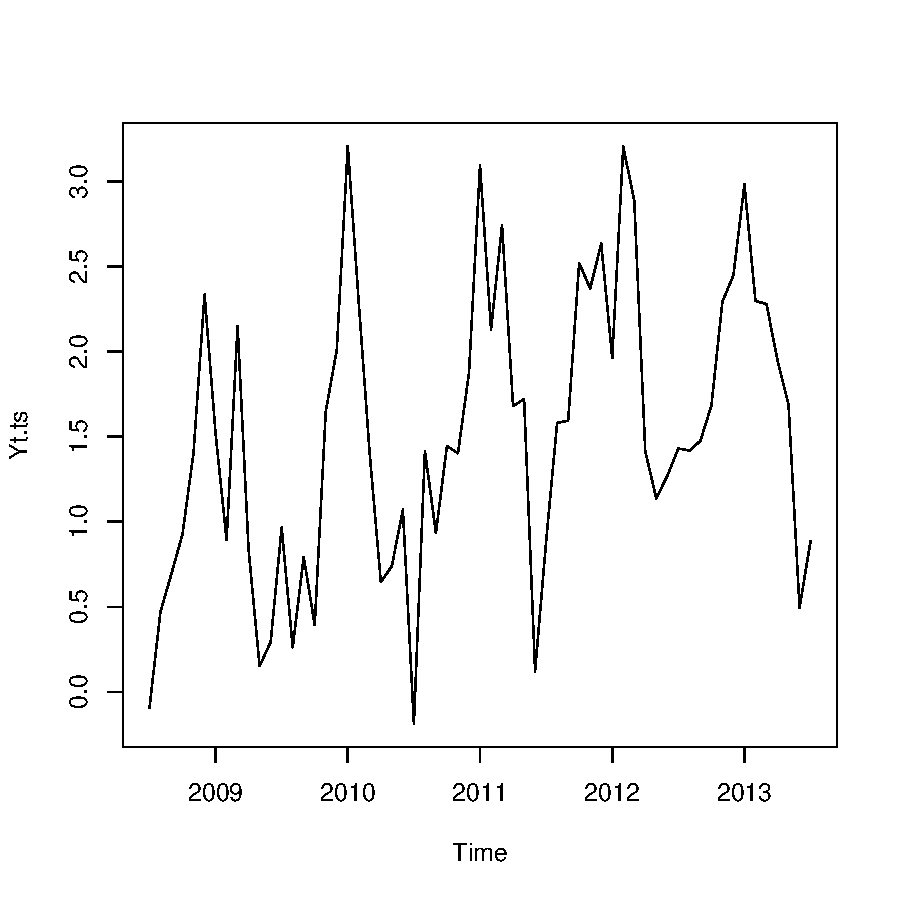
\includegraphics[height=4in, width=4in]{exercice1-graph1.pdf}
  \caption{Graphique de la série $Y_t$}
  \label{fig:exercice1-graph1}
\end{figure}

\textbf{Élimination de la saisonnalité}
\begin{Schunk}
\begin{Sinput}
> xtable(Zt.ts <- diff(Yt.ts,12),digits=1)
\end{Sinput}
% latex table generated in R 2.15.2 by xtable 1.7-1 package
% Sat Sep 21 21:11:36 2013
\begin{table}[ht]
\centering
\begin{tabular}{rrrrrrrrrrrrr}
  \hline
 & Jan & Feb & Mar & Apr & May & Jun & Jul & Aug & Sep & Oct & Nov & Dec \\ 
  \hline
2009 &  &  &  &  &  &  & 1.1 & -0.2 & 0.1 & -0.5 & 0.2 & -0.3 \\ 
  2010 & 1.7 & 1.4 & -0.8 & -0.2 & 0.6 & 0.8 & -1.2 & 1.2 & 0.1 & 1.1 & -0.2 & -0.1 \\ 
  2011 & -0.1 & -0.2 & 1.4 & 1.0 & 1.0 & -0.9 & 1.1 & 0.2 & 0.7 & 1.1 & 1.0 & 0.8 \\ 
  2012 & -1.1 & 1.1 & 0.1 & -0.3 & -0.6 & 1.1 & 0.5 & -0.2 & -0.1 & -0.8 & -0.1 & -0.2 \\ 
  2013 & 1.0 & -0.9 & -0.6 & 0.5 & 0.5 & -0.8 & -0.5 &  &  &  &  &  \\ 
   \hline
\end{tabular}
\end{table}\end{Schunk}

\begin{figure}[p]
  \centering
  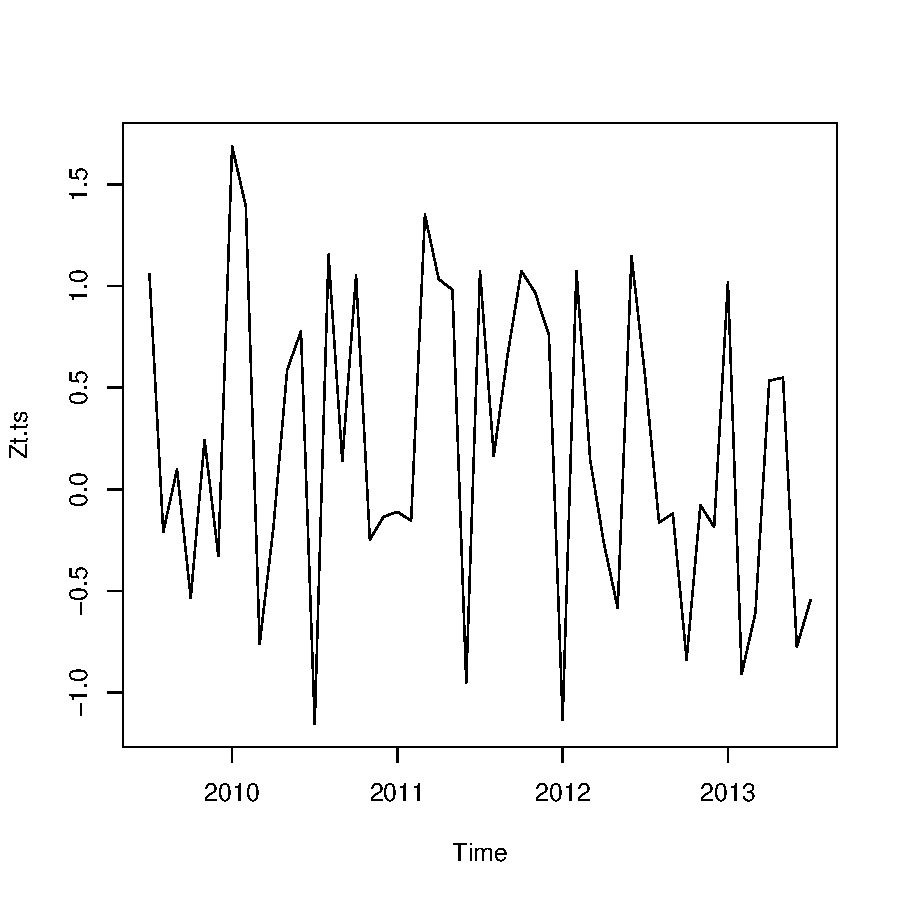
\includegraphics[height=4in, width=4in]{exercice1-graph2.pdf}
  \caption{Graphique de la série désaisonnalisée $Z_t$}
  \label{fig:exercice1-graph2}
\end{figure}

\textbf{Composante de saisonnalité}
\begin{Schunk}
\begin{Sinput}
> xtable(Yt.ts-Zt.ts,digits=1)
\end{Sinput}
% latex table generated in R 2.15.2 by xtable 1.7-1 package
% Sat Sep 21 21:11:36 2013
\begin{table}[ht]
\centering
\begin{tabular}{rrrrrrrrrrrrr}
  \hline
 & Jan & Feb & Mar & Apr & May & Jun & Jul & Aug & Sep & Oct & Nov & Dec \\ 
  \hline
2009 &  &  &  &  &  &  & -0.1 & 0.5 & 0.7 & 0.9 & 1.4 & 2.3 \\ 
  2010 & 1.5 & 0.9 & 2.2 & 0.8 & 0.2 & 0.3 & 1.0 & 0.3 & 0.8 & 0.4 & 1.6 & 2.0 \\ 
  2011 & 3.2 & 2.3 & 1.4 & 0.6 & 0.7 & 1.1 & -0.2 & 1.4 & 0.9 & 1.4 & 1.4 & 1.9 \\ 
  2012 & 3.1 & 2.1 & 2.7 & 1.7 & 1.7 & 0.1 & 0.9 & 1.6 & 1.6 & 2.5 & 2.4 & 2.6 \\ 
  2013 & 2.0 & 3.2 & 2.9 & 1.4 & 1.1 & 1.3 & 1.4 &  &  &  &  &  \\ 
   \hline
\end{tabular}
\end{table}\end{Schunk}

\begin{figure}[p]
  \centering
  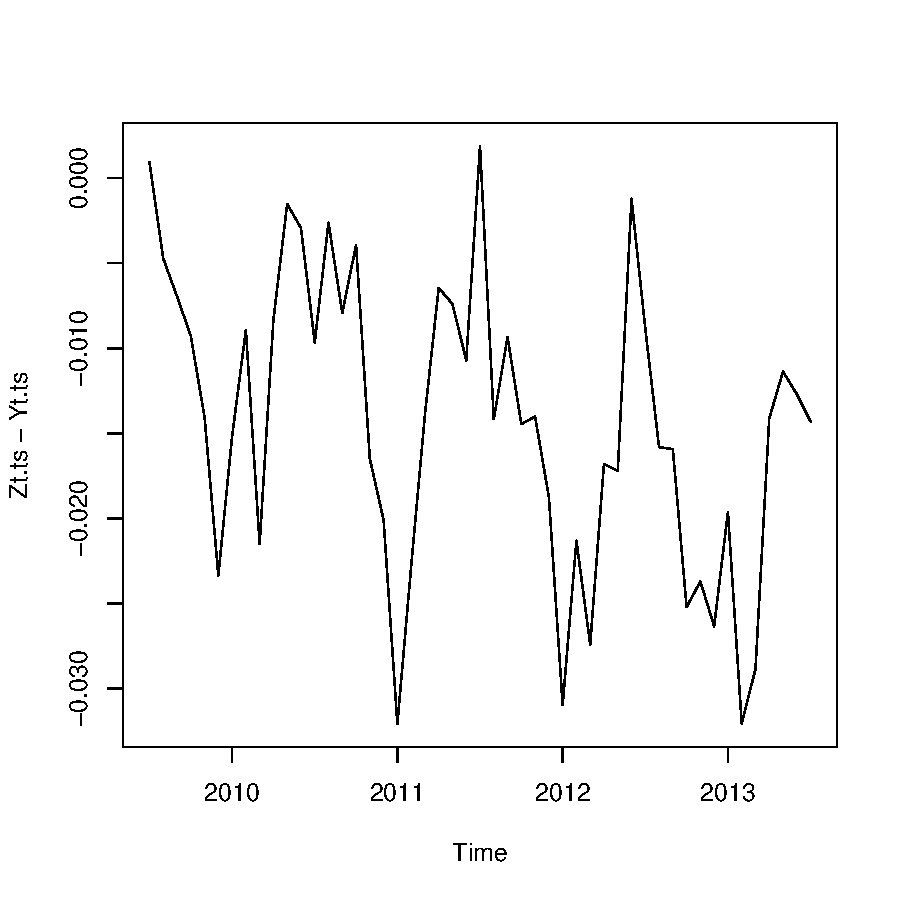
\includegraphics[height=4in, width=4in]{exercice1-graph3.pdf}
  \caption{Graphique de la composante de saisonnalité $Y_t-Z_t$}
  \label{fig:exercice1-graph3}
\end{figure}
\clearpage
\textbf{Élimination de la tendance}

Moyenne mobile avec $q=1$
\begin{Schunk}
\begin{Sinput}
> xtable(mt1 <- lag(SMA(Zt.ts,n=3),1),digits=2)
\end{Sinput}
% latex table generated in R 2.15.2 by xtable 1.7-1 package
% Sat Sep 21 21:11:36 2013
\begin{table}[ht]
\centering
\begin{tabular}{rrrrrrrrrrrrr}
  \hline
 & Jan & Feb & Mar & Apr & May & Jun & Jul & Aug & Sep & Oct & Nov & Dec \\ 
  \hline
2009 &  &  &  &  &  &  &  & 0.32 & -0.22 & -0.06 & -0.21 & 0.54 \\ 
  2010 & 0.92 & 0.77 & 0.15 & -0.12 & 0.39 & 0.07 & 0.26 & 0.05 & 0.78 & 0.32 & 0.22 & -0.16 \\ 
  2011 & -0.13 & 0.36 & 0.74 & 1.12 & 0.36 & 0.37 & 0.10 & 0.63 & 0.63 & 0.90 & 0.93 & 0.20 \\ 
  2012 & 0.23 & 0.03 & 0.32 & -0.24 & 0.10 & 0.37 & 0.51 & 0.09 & -0.37 & -0.34 & -0.37 & 0.25 \\ 
  2013 & -0.02 & -0.16 & -0.33 & 0.16 & 0.10 & -0.26 &  &  &  &  &  &  \\ 
   \hline
\end{tabular}
\end{table}\end{Schunk}
\clearpage 
Moyenne mobile avec $q=5$
\begin{Schunk}
\begin{Sinput}
> xtable(mt2 <- lag(SMA(Zt.ts,n=11),5),digits=2)
\end{Sinput}
% latex table generated in R 2.15.2 by xtable 1.7-1 package
% Sat Sep 21 21:11:36 2013
\begin{table}[ht]
\centering
\begin{tabular}{rrrrrrrrrrrrr}
  \hline
 & Jan & Feb & Mar & Apr & May & Jun & Jul & Aug & Sep & Oct & Nov & Dec \\ 
  \hline
2009 &  &  &  &  &  &  &  &  &  &  &  & 0.28 \\ 
  2010 & 0.25 & 0.17 & 0.26 & 0.32 & 0.40 & 0.40 & 0.24 & 0.10 & 0.16 & 0.30 & 0.34 & 0.36 \\ 
  2011 & 0.37 & 0.37 & 0.37 & 0.33 & 0.45 & 0.55 & 0.63 & 0.54 & 0.52 & 0.44 & 0.32 & 0.36 \\ 
  2012 & 0.36 & 0.40 & 0.32 & 0.22 & 0.05 & -0.02 & 0.06 & 0.06 & -0.04 & -0.07 & 0.03 & -0.02 \\ 
  2013 & -0.14 & -0.18 &  &  &  &  &  &  &  &  &  &  \\ 
   \hline
\end{tabular}
\end{table}\end{Schunk}
\clearpage 
Lissage exponentiel double avec $\alpha=0.75$
\begin{Schunk}
\begin{Sinput}
> xtable(mt3 <- DEMA(Zt.ts,n=1,ratio=.05),digits=2)
\end{Sinput}
% latex table generated in R 2.15.2 by xtable 1.7-1 package
% Sat Sep 21 21:11:36 2013
\begin{table}[ht]
\centering
\begin{tabular}{rrrrrrrrrrrrr}
  \hline
 & Jan & Feb & Mar & Apr & May & Jun & Jul & Aug & Sep & Oct & Nov & Dec \\ 
  \hline
2009 &  &  &  &  &  &  & 1.06 & 0.94 & 0.85 & 0.71 & 0.66 & 0.55 \\ 
  2010 & 0.65 & 0.72 & 0.57 & 0.48 & 0.48 & 0.50 & 0.33 & 0.39 & 0.36 & 0.41 & 0.33 & 0.28 \\ 
  2011 & 0.22 & 0.17 & 0.27 & 0.33 & 0.38 & 0.24 & 0.31 & 0.29 & 0.31 & 0.38 & 0.43 & 0.45 \\ 
  2012 & 0.29 & 0.36 & 0.33 & 0.26 & 0.17 & 0.25 & 0.27 & 0.22 & 0.18 & 0.07 & 0.04 & 0.01 \\ 
  2013 & 0.09 & -0.02 & -0.09 & -0.04 & 0.00 & -0.09 & -0.14 &  &  &  &  &  \\ 
   \hline
\end{tabular}
\end{table}\end{Schunk}
\clearpage 
Régression linéaire
\begin{Schunk}
\begin{Sinput}
> t <- 0:48
> (lm1 <- lm(Zt.ts~t))
\end{Sinput}
\begin{Soutput}
Call:
lm(formula = Zt.ts ~ t)

Coefficients:
(Intercept)            t  
    0.44692     -0.00986  
\end{Soutput}
\begin{Sinput}
> coeff1 <- coefficients(lm1)
\end{Sinput}
\end{Schunk}
\begin{Schunk}
\begin{Sinput}
> xtable(mt4 <- ts(coeff1[1]+t*coeff1[2],start=c(2009,7),deltat=1/12),digits=2)
\end{Sinput}
% latex table generated in R 2.15.2 by xtable 1.7-1 package
% Sat Sep 21 21:11:36 2013
\begin{table}[ht]
\centering
\begin{tabular}{rrrrrrrrrrrrr}
  \hline
 & Jan & Feb & Mar & Apr & May & Jun & Jul & Aug & Sep & Oct & Nov & Dec \\ 
  \hline
2009 &  &  &  &  &  &  & 0.45 & 0.44 & 0.43 & 0.42 & 0.41 & 0.40 \\ 
  2010 & 0.39 & 0.38 & 0.37 & 0.36 & 0.35 & 0.34 & 0.33 & 0.32 & 0.31 & 0.30 & 0.29 & 0.28 \\ 
  2011 & 0.27 & 0.26 & 0.25 & 0.24 & 0.23 & 0.22 & 0.21 & 0.20 & 0.19 & 0.18 & 0.17 & 0.16 \\ 
  2012 & 0.15 & 0.14 & 0.13 & 0.12 & 0.11 & 0.10 & 0.09 & 0.08 & 0.07 & 0.06 & 0.05 & 0.04 \\ 
  2013 & 0.03 & 0.02 & 0.01 & 0.00 & -0.01 & -0.02 & -0.03 &  &  &  &  &  \\ 
   \hline
\end{tabular}
\end{table}\end{Schunk}
\clearpage 
\begin{figure}[p]
  \centering
  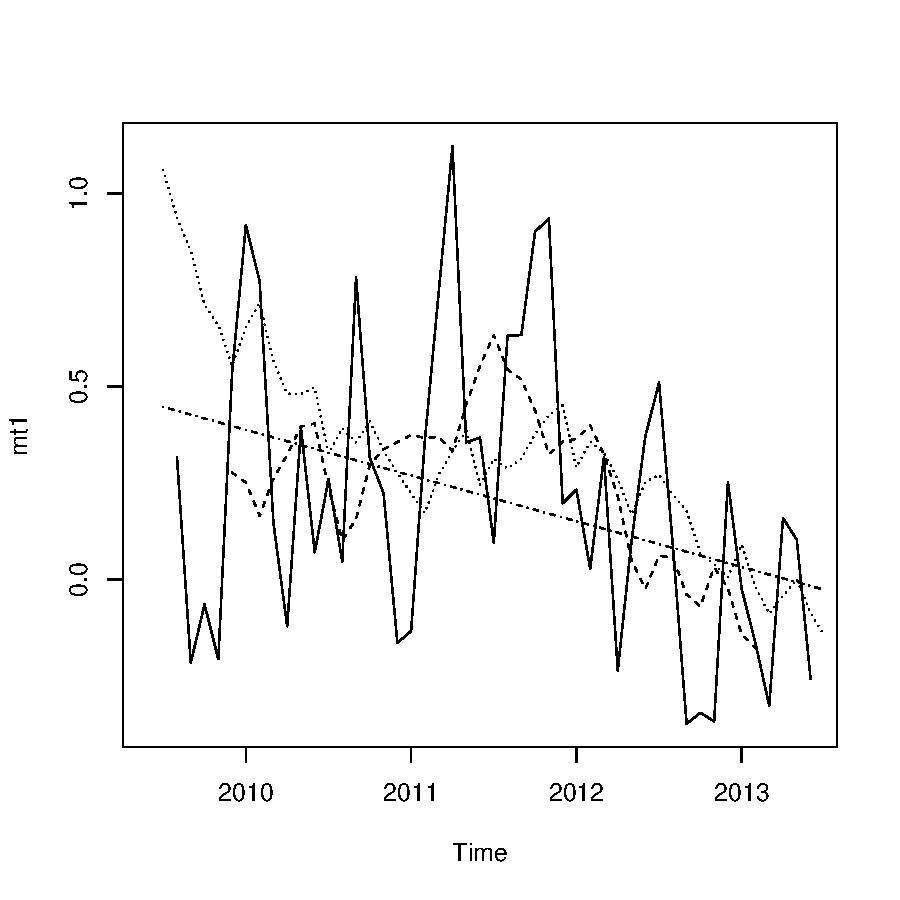
\includegraphics[height=4in, width=4in]{exercice1-graph4.pdf}
  \caption{Graphique de la tendance $m_t$}
  \label{fig:exercice1-graph4}
\end{figure}
\clearpage 
\textbf{Projection du taux d'inflation}
\begin{Schunk}
\begin{Sinput}
> projection <- coeff1[1]+53*coeff1[2]
> saisonnalite <- mean((Yt.ts-Zt.ts)[6+12*0:3])
> (taux.inf.dec.2013 <- (projection+saisonnalite))
\end{Sinput}
\begin{Soutput}
(Intercept) 
      2.138 
\end{Soutput}
\end{Schunk}
Le taux d'inflation prejeté en décembre 2013 est 2.14\%\\

\textbf{Solution du problème}
\begin{Schunk}
\begin{Sinput}
> depense.dec.2008 <- 674
> depense.dec.2013 <- 674*(1+taux.inf.dec.2013/100)
\end{Sinput}
\end{Schunk}
Le montant projeté des achats de cadeaux en décembre 2013 est 688.41 \$

\clearpage 
\subsection{Incendies}

On remarque d'abord que $q=2$.

On peut ensuite poser les équations suivantes:
\begin{align}
  \label{eq:1}
  4+3+a+b+2 &= 24\\
  b+2+4+6+c &= 26\\
  c+0+2+8+3 &= 19
\end{align}

En résolvant, on obtient la solution.\\

\textbf{Solution:}\\

\begin{tabular}{|l|l|l|}
\hline
\multicolumn{1}{|l|}{Mois} & \multicolumn{1}{l|}{Incendies} & \multicolumn{1}{l|}{Moyenne Mobile} \\ \hline
1 & 4 & \multicolumn{1}{l|}{-} \\ \hline
2 & 3 & \multicolumn{1}{l|}{-} \\ \hline
3 & \textbf{7} & 4,8 \\ \hline
4 & \textbf{8} & 4,8 \\ \hline
5 & 2 & 5,4 \\ \hline
6 & 4 & 5,2 \\ \hline
7 & 6 & 3,6 \\ \hline
8 & \textbf{6} & 3,6 \\ \hline
9 & 0  & 4,4 \\ \hline
10 & 2 & 3,8 \\ \hline
11 & 8 & \multicolumn{1}{l|}{-} \\ \hline
12 & 3 & \multicolumn{1}{l|}{-} \\ \hline
\end{tabular}

\clearpage

\subsection{Option de vente}

\begin{Schunk}
\begin{Sinput}
> rf <- 0.0175
> rB <- rf+0.02
> S0 <- 10.46
> ST <- 8.73
> K <- S0*exp(rf*84/365)
> bbry <- read.csv("blackberry.csv",header=TRUE,sep=";")
> bbry.sel <- bbry[as.POSIXlt(bbry$Date)$wday==5,][1+3:12*4,]$Close 
>                                         #Extraire le prix un vendredi sur 4
> l.bbry.sel <- log(bbry.sel)
> (diff.l.bbry.sel <- diff(l.bbry.sel)) 
\end{Sinput}
\begin{Soutput}
[1]  0.288638  0.112996 -0.061345 -0.103096 -0.017498 -0.086523  0.005008
[8] -0.340979 -0.090637
\end{Soutput}
\begin{Sinput}
>                                         #On obtient la série des rendements
>                                         #mensuels
> (mu.diff.l.bbry.sel <- mean(diff.l.bbry.sel))
\end{Sinput}
\begin{Soutput}
[1] -0.0326
\end{Soutput}
\begin{Sinput}
> (sigma.diff.l.bbry.sel <- sd(diff.l.bbry.sel))
\end{Sinput}
\begin{Soutput}
[1] 0.1707
\end{Soutput}
\begin{Sinput}
>                                         #Moyenne et écart-type des rendements 
>                                         #mensuels
> (prix.arbre <- S0*(ud <- exp(3*(mu.diff.l.bbry.sel+c(1,-1)*
+                                 sigma.diff.l.bbry.sel/(2*sqrt(3))))))
\end{Sinput}
\begin{Soutput}
[1] 10.997  8.182
\end{Soutput}
\begin{Sinput}
>                                         #Prix de l'arbre binomial
> (p.rn <- (exp(rf*84/365)-ud[2])/(ud[1]-ud[2]))
\end{Sinput}
\begin{Soutput}
[1] 0.8243
\end{Soutput}
\begin{Sinput}
>                                         #Probabilité neutre au risque
> q.rn <- 1-p.rn
> (P0 <- sum(exp(-rf*84/365)*(c(p.rn,q.rn)*pmax(K-prix.arbre,0))))
\end{Sinput}
\begin{Soutput}
[1] 0.4061
\end{Soutput}
\begin{Sinput}
>                                         #Prix de l'option de vente
> (BT <- P0*exp(rB*84/365)) #Montant emprunté avec intérêts
\end{Sinput}
\begin{Soutput}
[1] 0.4096
\end{Soutput}
\begin{Sinput}
> (K-ST)-BT  #Profit
\end{Sinput}
\begin{Soutput}
[1] 1.363
\end{Soutput}
\end{Schunk}

La valeur du paramètre $\mu$ de rendement moyen est -0.0326.
La valeur du paramètre $\sigma$ de volatilité est 0.1707.
La valeur des prix de l'arbre binomial sont 10.9968 et 8.1816.
La valeur de la probabilité neutre au risque d'une hausse est 0.8243.
La valeur de l'option est 0.4061.
Le profit, qui correspont à la différence entre la réclamation contingente de l'option et le coût d'acquisition, est de 1.3626.

\clearpage

Document généré le \today \ à \ \thistime 

\clearpage


\includegraphics[height=7mm,keepaspectratio=true]{by-sa}\\
Cette création est mise à disposition selon le contrat
\href{http://creativecommons.org/licenses/by-sa/2.5/ca/deed.fr}{%
  Paternité-Partage à l'identique 2.5 Canada} de Creative Commons
disponible à l'adresse \\
http://creativecommons.org/licenses/by-sa/2.5/ca/deed.fr \\
En vertu de ce contrat, vous êtes libre de:
\begin{itemize}
\item \textbf{partager} --- reproduire, distribuer et communiquer
  l'{\oe}uvre;
\item \textbf{remixer} --- adapter l'{\oe}uvre;
\item utiliser cette {\oe}uvre à des fins commerciales.
\end{itemize}
Selon les conditions suivantes:

  \begin{tabularx}{\linewidth}{@{}lX@{}}
    \raisebox{-9mm}[0mm][13mm]{%
      
\includegraphics[height=11mm,keepaspectratio=true]{by}} &
    \textbf{Attribution} --- Vous devez attribuer l'{\oe}uvre de la
    manière indiquée par l'auteur de l'{\oe}uvre ou le titulaire des
    droits (mais pas d'une manière qui suggérerait qu'ils vous
    soutiennent ou
    approuvent votre utilisation de l'{\oe}uvre). \\
    \raisebox{-9mm}{
\includegraphics[height=11mm,keepaspectratio=true]{sa}}
    & \textbf{Partage à l'identique} --- Si vous modifiez, transformez
    ou adaptez cette {\oe}uvre, vous n'avez le droit de distribuer
    votre création que sous une licence identique ou similaire à
    celle-ci.
  \end{tabularx}
\end{document}
